% @name manual.tex
% @note analysis software manual
% @author firdaus janoos
% @date Friday, April 15, 2011 at 12:10
%%%%%%%%%%%%%%%%%%%%%%%%%%%%%%%%%%%%%%%%%%%%%%%%%%%%%%%%%%%%%%%%%%%%%%%%%%%%%%%

\documentclass{book}
%
% To change the dissertation to a Master's Thesis, include a documentclass
% option such as [masters], [ms], [ma], etc.  Also available are [osudraft]
% and [twoside].  As a reminder, documentclass options are a
% comma-separated list, e.g. \documentclass[ms,osudraft]{osudissert96}
%

fj/preamble.tex


% BibTeX from the BiBTeX Documentation
\def\BibTeX{{\rm B\kern-.05em{\sc i\kern-.025em b}\kern-.08em
    T\kern-.1667em\lower.7ex\hbox{E}\kern-.125emX}}

%
% It is better to break up the dissertation into multiple files (e.g.,
% one file per chapter, as well as separate files for the abstract,
% acknowledgements, and vita).  These files are brought into the
% document using \include{} statements.  There will be times, however,
% when you don't want to print the ENTIRE dissertation.  You can limit
% what will actually be printed by using the \includeonly{} statment.
% This contains a list of the files you want printed.  Any file NOT
% listed will not be printed.  However, all page numbers, references,
% etc., will be preserved as though all the files were actually
% printed. For example, the line below would result only in chapters 1
% and 3 being printed (if it were uncommented).
%
%\includeonly{ch1.intro,ch3.implem}

%  In the new format, the titles of each chapter should appear in
%  uppercase.  In the TOC, however, they should be in lowercase.
%  The command below automates this behavior.  However, you'll have to be
%  careful not to include \labels within your \chapter definitions or
%  there will be problems.  If you don't want this to be automated, comment
%  out the \typesetChapterTitle definition below and do your chapters in
%  the form:
%  \chapter[MY TITLE]{My Title}



% using chapterbib
\renewcommand\refname{REFERENCES}
\renewcommand\bibname{REFERENCES}

\graphicspath{{./figures/}}

\begin{document}


%------------------------------------------------------------------------------
% Title Pages
%------------------------------------------------------------------------------
%\title{Exploring the Temporal Dimension of fMRI}
\title{Spatio-Temporal State-Space Analysis for fMRI\\
\textbf{User Manual}}
\author{Firdaus Janoos} % insert your name


\maketitle


%------------------------------------------------------------------------------
% Main Content
%------------------------------------------------------------------------------

\tableofcontents
\listoffigures

\chapter{Introduction}
This manual describes the procedure for building and analyzing
spatio-temporal state-space models of neural processes. Please refer
to \citet{Janoos2011}. A flowchart depiction of the algorithm
developed in that paper is shown in \Fig{fig:pipeline}

\begin{figure}[h!]
\centering {
  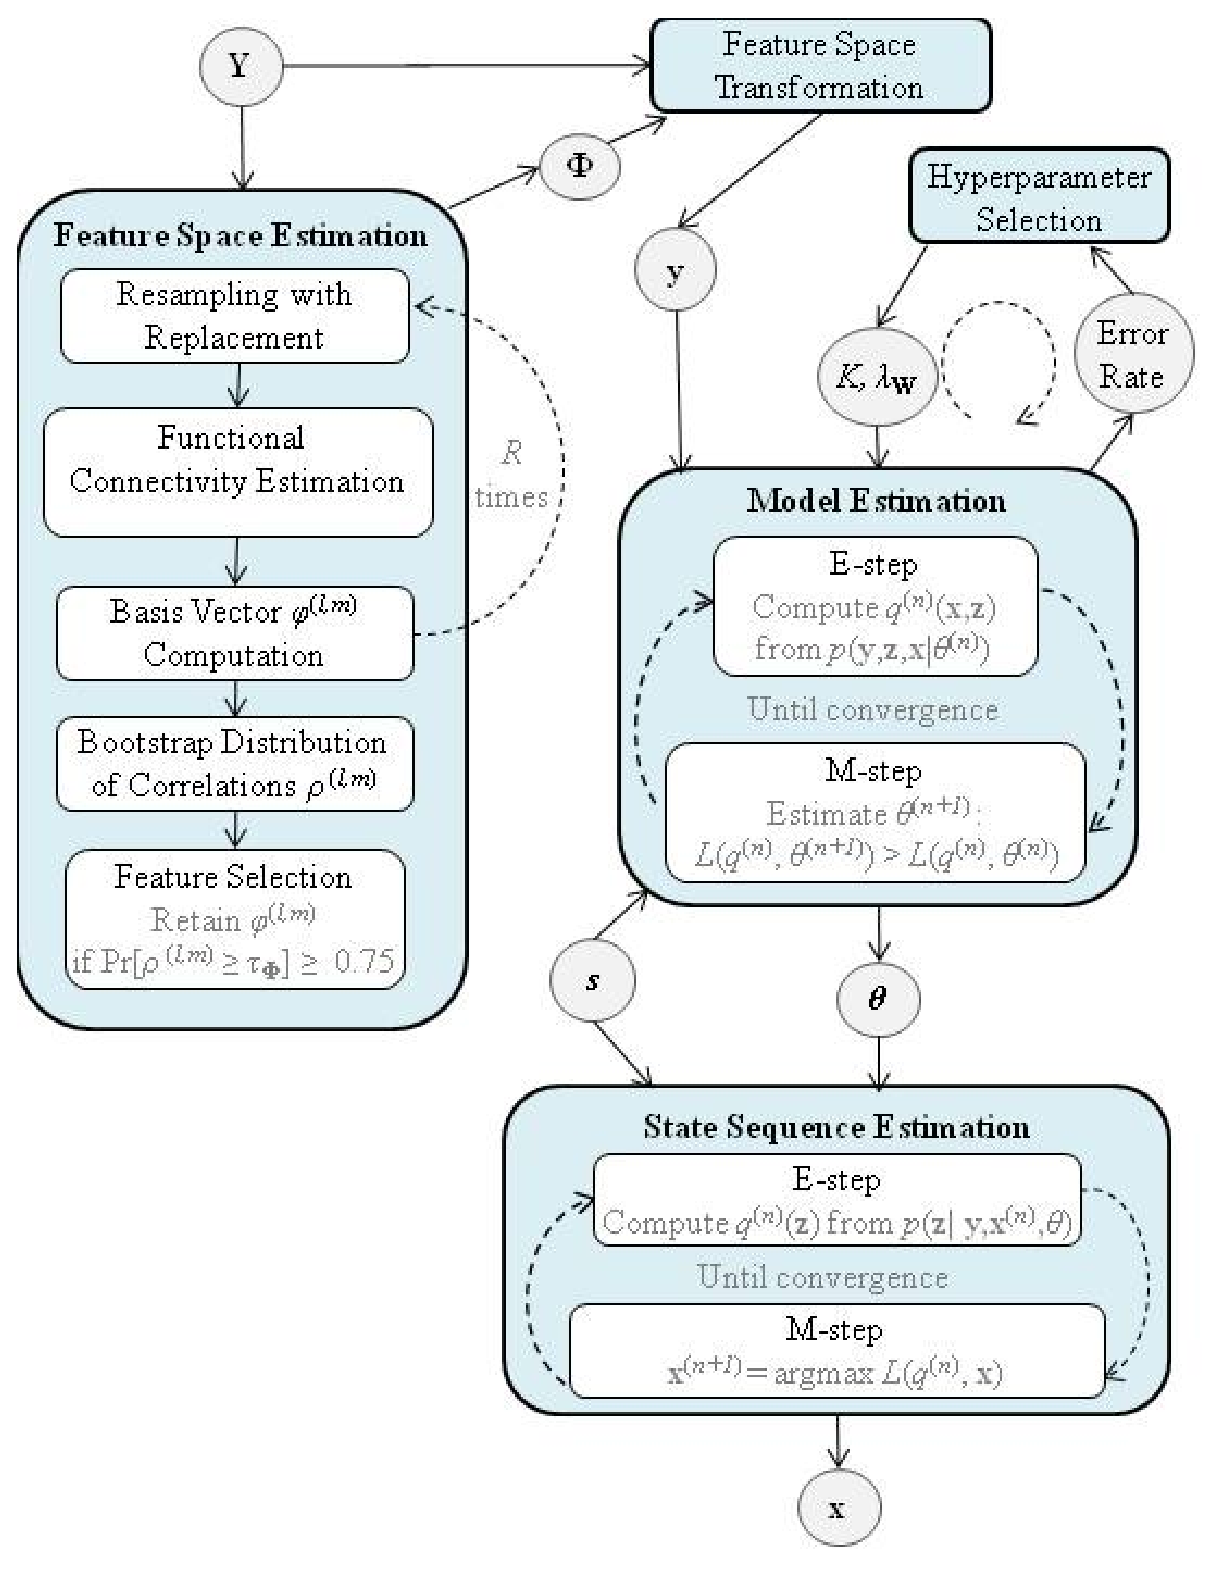
\includegraphics[width=0.8\linewidth]{pipeline-v2}}
  \caption[Outline of Method]{
  Basis vectors of the feature--space $\Phi$ are computed from the functional
  connectivity of the brain estimated from
  the fMRI data $\y$.  Dimensionality reduction is performed
  by retaining stable basis vectors using bootstrapping.
  The data ($\Y$), after projecting into the low dimensional feature--space
 are used to estimate model   parameters $\theta$ through a
  generalized EM algorithm.
  Model hyper--parameters $K$ and $\lambda_\w$ are selected
  to minimize the error of predicting the stimulus $\s$.
  Given a set of model parameters, the optimal
  state--sequence $\X^*$ is estimated using EM.
  }\label{fig:pipeline}
\end{figure}

This algorithm has been implemented in a combination of
MATLAB$^\circledR$ codes, MATLAB$^\circledR$ with
Star-P$^\circledR$, and \verb"C++".

\section{Single Session Analysis}
The main steps involved in analyzing a single session\footnote{That
is, to analyze one continuous fMRI time-series of one subject, one
session. It may consists of one actual run, or multiples runs
concatenated together. Essentially, one session is any fMRI
time-series that shares the same anatomy and imaging
characteristics.} data-set are:
\begin{enumerate}[i]
  \item Preprocessing for
  \begin{enumerate}
    \item Slice timing correction
    \item Head motion correction
    \item De-noising
    \item Head motion artifact removal
    \item Other signal artifact removal (e.g. scanner drift, pulsatile signal, respiratory signal)
  \end{enumerate}
  \item Building the feature space
  \item Specifying the experimental design
  \item Model estimation
  \item Model exploration
\end{enumerate}

\section{Multi-Subject Analysis}
In addition to the steps required for a single session analysis,
during the preprocessing step  data is spatially normalized into a
reference coordinate system using non-linear registration.

Group level analysis is performed by comparing the models across
subjects, in terms of state-space behavior and spatial activation
patterns.

\section{Prerequisites}

\subsection{Hardware}
A really fast computer / workstation to examine and explore the
results. Access to a kick-ass cluster to do the heavy duty
computation.

\subsection{Software}
\begin{enumerate}
  \item MATLAB$^\circledR$ on the work-station for design
  specification and results exploration.
  \item MATLAB$^\circledR$ with Star-P$^\circledR$ installed and
  configured, for feature-space computation and model estimation.
  \item SPM~\cite{TheFILMethodsGroup2011} version 5 or higher
  \item Group ICA of fMRI Toolbox (GIFT) \footnote{\url{http://icatb.sourceforge.net/gift}} version 1.2 or higher.
  \item An ISO Standard compatible C++ compiler.
  \item ITK\cite{Ibanez2003} version 2 or higher, installed and configured.
\end{enumerate}


\chapter{Preprocessing}
Each data-set will have different artifacts and characteristics and
the pre-processing should be adapted to it. However, in general we
have the following procedure to be effective in order for further
spatio-temporal modeling.

In the discussion that follows, each session (run) is pre-processed
individually.

\section{Slice Timing and Motion Correction with SPM}
\label{sec:slc-tim}

\begin{figure}
    \begin{center}
   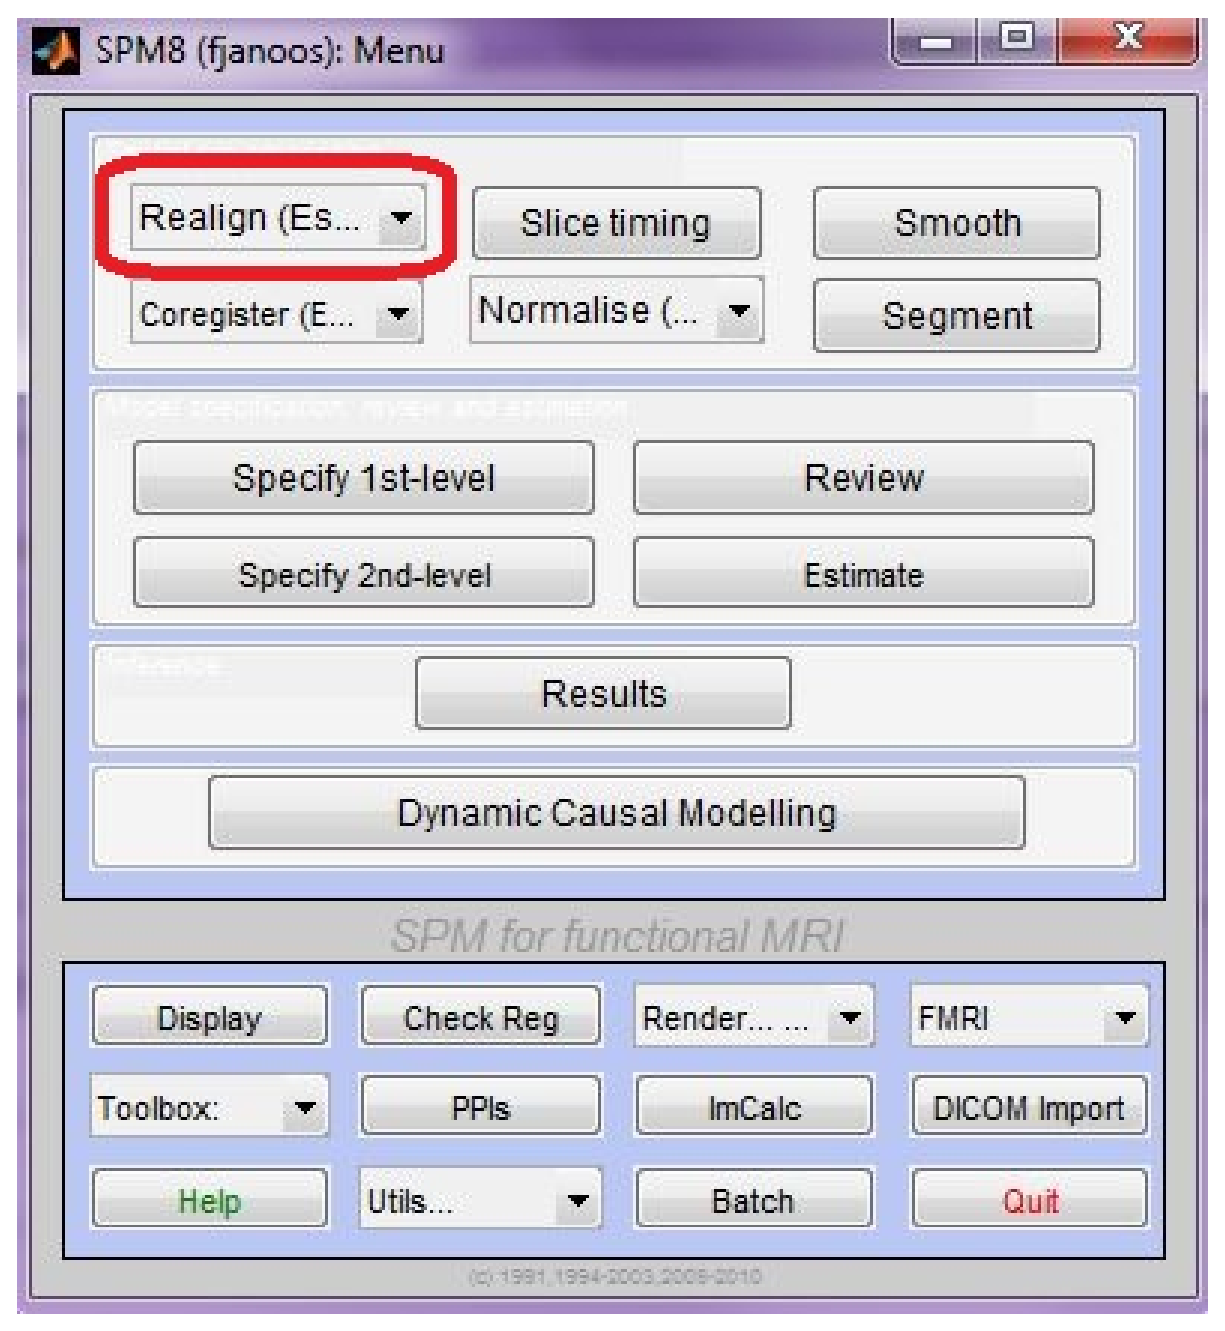
\includegraphics[width=.37\linewidth]{figures/spm-est_res}
    \caption[Estimate and Reslice Option of SPM8.]
    {Estimate and Reslice Option of SPM8.\label{fig:spm-est_res}}
    \end{center}
\end{figure}
Use the slice timing and motion correction modules from SPM5. For
motion correction, apply the \verb"Estimate and Reslice" operations
(\cf~\Fig{fig:spm-est_res}).

In order to remove residual motion artifacts from the time-series
data (described in the next section), build a design matrix
consisting only of the motion parameters estimated by SPM
(\verb"rp_*.txt"), and save it as an \verb"SPM.mat" file\footnote{By
selecting the file in the { Multiple Regressors} field of the SPM {
Specify 1st-level} GUI. Do not include regressors for any
experimental conditions}.

For details, refer to the SPM Manual\cite{TheFILMethodsGroup2011}.

\section{Motion Artifact Removal with GIFT}

\begin{figure}
    \begin{center}
   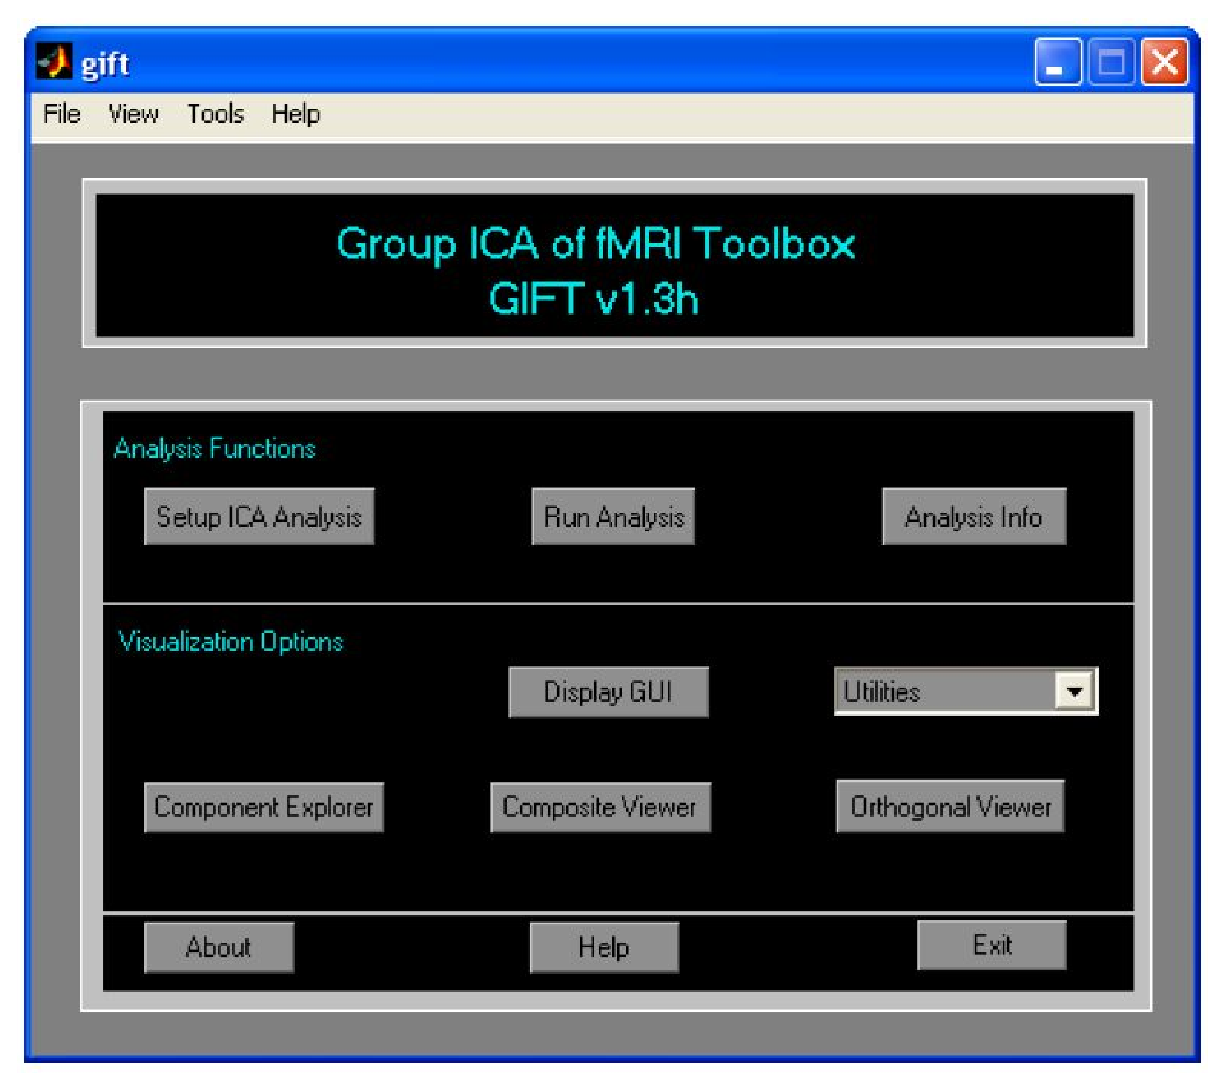
\includegraphics[width=.5\linewidth]{figures/gift}
    \caption[Group ICA for fMRI Toolbox (GIFT)]
    {Group ICA for fMRI Toolbox (GIFT).
     \label{fig:gift}}
    \end{center}
\end{figure}
The motion correction operation itself tends to introduce strong
artifacts \citet{Grootoonk2000}. These artifacts are removed using
ICA analysis with GIFT (\cf~\Fig{fig:gift}). For this, first start
up GIFT and configure it for analysis of an individual
session(\cf~\Fig{fig:gift-setup}). Set the number of ICA to that
automatically estimated by GIFT. Set ICA Algorithm to Infomax and
Group ICA Analysis to Regular. Use the setup defaults for all other
settings.

\begin{figure}
    \begin{center}
   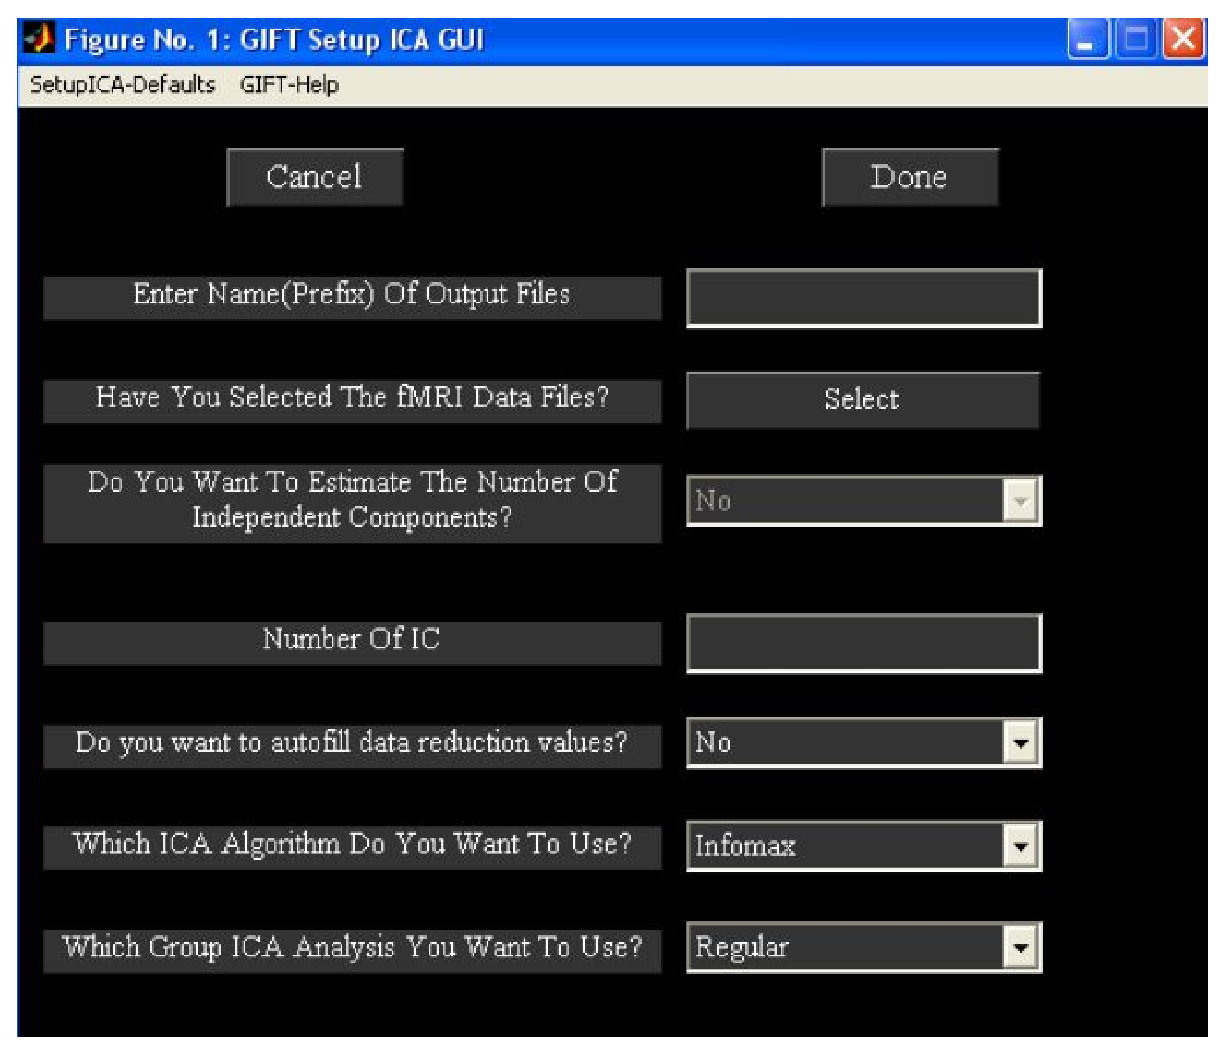
\includegraphics[width=.5\linewidth]{figures/gift-ica-setup}
    \caption[Configuring a GIFT analysis session.]
    {Configuring a GIFT analysis session.
     \label{fig:gift-setup}}
    \end{center}
\end{figure}

After configuring the GIFT analysis, run all the analysis steps
\begin{figure}
    \begin{center}
   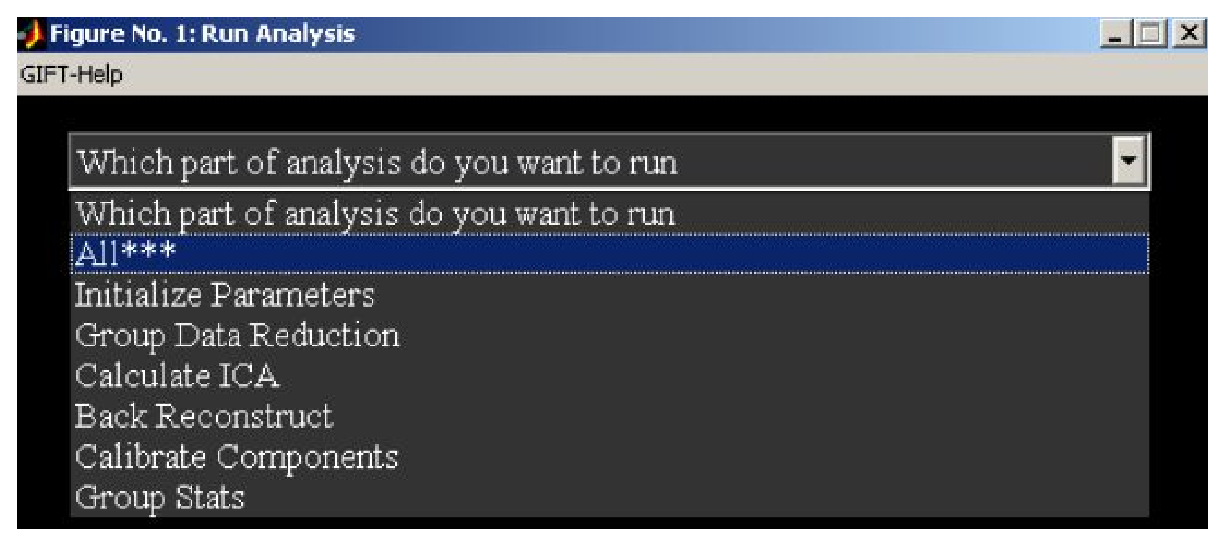
\includegraphics[width=.5\linewidth]{figures/gift-run}
    \caption[Group ICA for fMRI Toolbox (GIFT).]{Group ICA for fMRI Toolbox (GIFT).
     \label{fig:gift-setup}}
    \end{center}
\end{figure}

After the analysis is complete, open the \verb"Component Explorer"
and select the generated parameter file. Now, identify components of
artifactual origin using one of two methods:

\begin{enumerate}[a]
  \item Manual inspection of components for high concentration of
  intensity close to vessicles, tissue interfaces and image
  boundaries.
  \item Sorting component through multiple regression against motion
  parameters estimated in \Sec{sec:slc-tim}. This can be
  achieved the \verb"Sort Components" feature of the visualization
  GUI and providing the design matrix of the SPM.mat file containing
  regressors built from the motion parameters (\cf~\Fig{fig:gift-regress}).
\end{enumerate}

\begin{figure}
    \begin{center}
   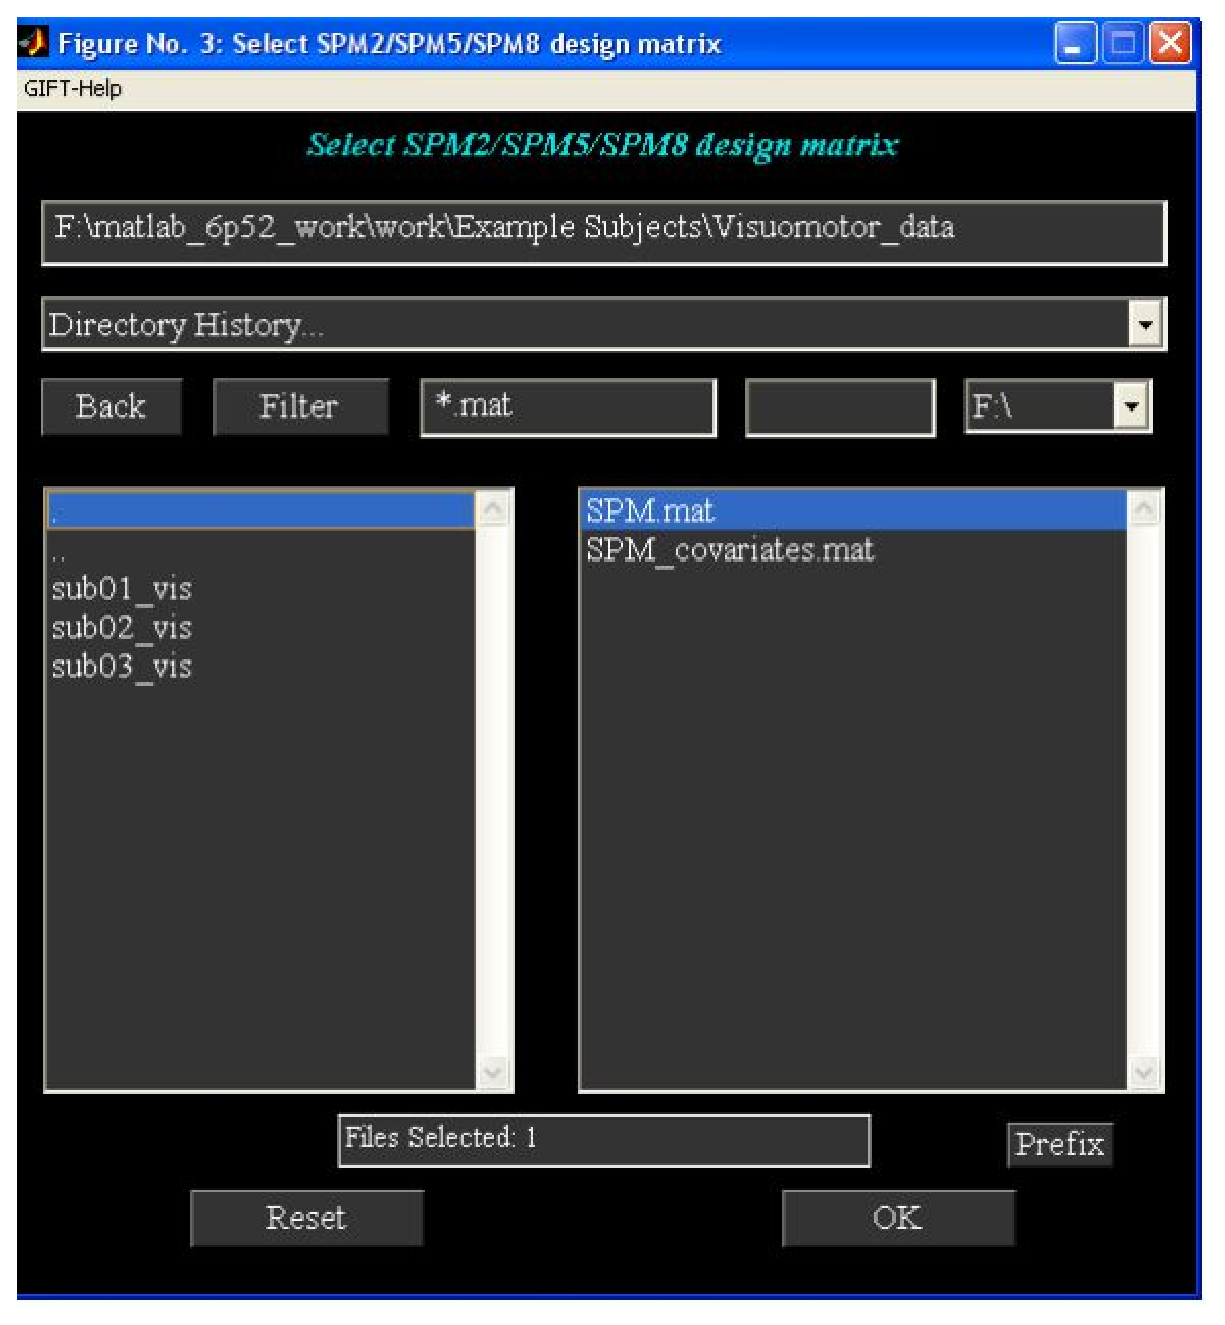
\includegraphics[width=.37\linewidth]{figures/gift-regress}
    \caption{Sorting components through regression in GIFT.
     \label{fig:gift-regress}}
    \end{center}
\end{figure}

After the artifactual components have been identified, they can be
effectively removed from the time-series data through the \verb"Back Reconstruction"
facility available in GIFT.

Please refer to the GIFT manual for more details.

\section{De-noising}

The preferred method of removing random $1/f$--type noise present in the fMRI time-course data
is a wavelet based algorithm \cite{Alexander2000}, that used a Wiener-type shrinkage for thresholding
noise coefficient.

For this, the steps are as follows, in MATLAB\footnote{Make sure to use a copy of the original data, as this
routine will overwrite the volumes in the vi structure.}:
\begin{verbatim}
    \% load the fmri dataset
    vi = spm_vol( epi_series_copy_fnames );
    preprocWaveletDenoise(vi, 'daubechies', 'wiener');
\end{verbatim}

The options for
\begin{verbatim}
preprocWaveletDenoise( epi\_vol\_info\_struct,
 wavelet\_type, shrinkage\_type )
\end{verbatim}
are:
\begin{itemize}
  \item \verb"epi\_vol\_info\_struct" - the array of \verb"spm\_vol" structures of the EPI time-series. Note that the
  files pointed to by these structures are used both as input and output of the denoising routine.
  \item \verb"wavelet\_type" - Valid choices are \verb"daubechies", \verb"haar", or \verb"cdf97".
  \item \verb"shrinkage\_type" - Valid options are \verb"hard", \verb"soft", \verb"sure", \verb"wiener".
\end{itemize}

Next, the time--series data are high-pass filtered ($0.5$Hz) to remove artifacts due
to breathing, blood pressure changes and scanner drift. Further polynomial trends are also eliminated through
polynomial regression\footnote{The method uses a complex analytic representation of the signal and of
a Legendre polynomial basis for regression.}.

For this, use the same \verb"spm\_vol" structure array obtained from above as input to
\begin{verbatim}
preprocDetrend( epi\_vol\_info\_struct,
freq\_cutoff, poly\_order )
\end{verbatim}
are:
\begin{itemize}
  \item \verb"epi\_vol_info_struct" - the array of \verb"spm\_vol" structures of the EPI time-series. Note that the
  files pointed to by these structures are used both as input and output of the denoising routine.
  \item \verb"freq\_cutoff" - The upper frequency for truncation.
  \item \verb"poly\_order" - The highest order of the polynomial for detrending.
\end{itemize}
%
%TODO: The frequency filtering and polynomial detrending can also be done in the wavelet basis. Need to integrate them into
%the denoising step.


\chapter{Feature Space Computation}
\label{chap:feature-space}
%feature-space.v1
As seen in \Fig{fig:pipeline}, computing the low-dimensional
feature-space representation of the data involves the following
steps:

\begin{enumerate}
  \item Generate a re-sample of the fMRI session.
  \item Compute the functional connectivity for the resample.
  \item Compute the orthogonal basis for the resample.
  \item Retain or discard basis vectors using bootstrap analysis of
  stability\cite{Bellec2010}.
  \item Project each fMRI volume (time-point) into the low
  dimensional feature space obtained above.
\end{enumerate}


The algorithms that provide this functionality are extremely
computation intensive though easily parallelized, and are therefore
implemented in MATLAB$^\circledR$ with Star-P$^\circledR$. To run
this module, it essential to have Star-P$^\circledR$ installed and
configured with MATLAB. Also, it is recommended that a cluster or
high-end high memory multi-processor computer be used. For an fMRI
session with $\approx 500$ volumes at $3$mm resolution, a minimum of
32GB RAM is essential.

A example of feature-space computation and projection operation code
fragment is:
\begin{verbatim}
    % load the preprocessed fMRI session
    vi_original = spm_vol( epi_series_preprocessed_fnames );
    % load a mask for the ROI
    vi_mask = spm_vol( roi_mask_fname);
    basis_filename = {};
    num_boot_iter = 1000;
    % BOOTSTRAP : iterate over multiple resamples
    for boot_iter = 1 : num_boot_iter
        % select a resample
        if boot_iter == 1
            % keep the first resample as the original sample
            vi_resample = vi_original;
        else
            [vi_resample] = fsResample( vi_original,
                                        ``block'', 10  );
        end
        % compute the connectivity matrix for the resample
        fsComputeConnectivity(vi_resample, vi_mask, 4,
                                0.25, connectivity_filename.bin);
        % compute the orthogonal basis vectors for the resample
        basis_filename{boot_iter} = [basis_filename_template,
                num2str(boot_iter)];
        fsOrthogonalize(connectivity_filename.bin,
                                basis_filename{boot_iter});
    end
    % perform the bootstrap analysis of stability
    [basis_set_idx, num_basis] =
                                fsBASC(basis_filename, 0.8, 0.75);
    % project original data on basis
    [basis_coords]=  fsProjectBasis( vi_original, basis_set_idx
                                        basis_filename{1});
\end{verbatim}

\section{Resampling the fMRI Session}
Function Syntax:
\begin{verbatim}
    [vi_resample] = fsResample( vi_original, resamp_type,
    option_1, option_2  );
\end{verbatim}
Arguments:
\begin{itemize}
  \item \verb"vi_original" - The array of \verb"spm_vol" structures of the original EPI time-series.
  \item \verb"resamp_type" - Valid choices are \verb"``block''" which selects the block bootstrap method
  described in \cite{Janoos2011} or   \verb"``wavelet''" that selects the wavelet based
  time-series bootstrapping method described in \cite{Patel2006}.
  \item \verb"option_1" - For \verb"resamp_type=``block''",
  \verb"option_1" is the length of a block in TR units. Typically
  \verb"option_1=10" has been found to be suitable for different
  datasets. The reader is referred to \cite{Janoos2010g} for more
  details on the tradeoffs involved. For
  \verb"resamp_type=``wavelet''", \verb"option_1" is the size of
  the coarsest scale in the wavelet decomposition tree, in TR units.
  Wavelet coefficients over a support greater than this value are
  not computed for permutation.
  \item \verb"option_2" - Not defined for
  \verb"resamp_type=``block''".
  For \verb"resamp_type=``wavelet''", \verb"option_2" is the order
  (number of vanishing moments) of the wavelet basis. A typical value is
  between 2 and 5.
\end{itemize}
Returns:
\begin{itemize}
  \item \verb"vi_resample" - The resample of the session.
\end{itemize}


\section{Computing Functional Connectivity for a Resample}
Function Syntax:
\begin{verbatim}
    fsComputeConnectivity( vi_resample, fwhm,
                        hac_frac, output_filename)
\end{verbatim}
Arguments:
\begin{itemize}
  \item \verb"fwhm" - The FWHM (in mm) of the Gaussian filter during the
  HAC step, typically set to 4.
  \item \verb"hac_frac" - The number of HAC clusters as a
  fraction of the number original voxels.
  \item \verb"output_filename" - The name of the output file
  in which to store the connectivity matrix. The matrix is
  stored row-wise in binary format (single precision float).
\end{itemize}
 Notes: This function is implemented in \verb"C++" with a
MATLAB hook.

\section{Computing the Orthogonal Basis Vectors}
Function Syntax:
\begin{verbatim}
    fsOrthogonalize(connectivity_filename_input,
                                basis_filename);
\end{verbatim}
Arguments:
\begin{itemize}
  \item \verb"connectivity_filename_input" -
    The file containing the connectivity matrix.
  \item \verb"basis_filename" - The file name (prefix) of
  the output files in which the basis vectors are stored (in zipped 4D NII
  format). Example, \verb"/data/session/subject_basis_resample_4"
  will result in the $N$ basis vectors   corresponding to the 4-th
  resample of the session being stored in the file
  \verb"/data/session/subject_basis_resample_4.nii.gz".
\end{itemize}


\section{Bootstrap Analysis of Stability}
\label{sec:basc}
 Function Syntax:
\begin{verbatim}
    [basis_set_idx, num_basis] =
                        fsBASC(basis_filename_array, tau, p);
\end{verbatim}
Arguments:
\begin{itemize}
  \item \verb"basis_filename_array" -
    A cell array of filenames of the 4D zipped NII (\verb".nii.gz")
    each containing the basis vectors computed for a resample of the
    session.
  \item \verb"tau" - The threshold at which correlations between the
  corresponding basis vectors across resamples are retained.
  Typically set between 0.6 and 0.9.
  \item \verb"p" - The probability value of suprathreshold correlations,
  if when exceeded the corresponding basis vector is retained in the
  final low-dimensional set.
\end{itemize}
Returns:
\begin{itemize}
  \item \verb"basis_set_idx" -
   The indices of the basis vector retained.
  \item \verb"num_basis" - The number of basis vectors retained
\end{itemize}

\section{Project Session on to Basis}
Function Syntax:
\begin{verbatim}
    [fs_coords]=  fsProjectBasis( vi_original,
                basis_set_idx, basis_filename);
\end{verbatim}
Arguments:
\begin{itemize}
    \item \verb"vi_original" - The array of \verb"spm_vol" structures of the original EPI time-series.
 \item \verb"basis_set_idx" -
   The indices of the basis vector retained.
  \item \verb"basis_filename" -
    The filename of the 4D zipped NII (\verb".nii.gz")
    containing the basis vectors computed for a particular re-sample of the
    session.
\end{itemize}
Returns:
\begin{itemize}
  \item \verb"fs_coords" - An number of scans times number of basis
  array giving the coordinates of each fMRI time-frame in the low
  dimensional feature space.
\end{itemize}


\chapter{Model Specification and Estimation}
%model-specify.v1

The state-space model (\cf.~\Fig{fig:model}) requires as input:
\begin{enumerate}
  \item The fMRI data (projected into the low-dimensional
  feature-space), described in \Chap{chap:feature-space}.
  \item Information about the stimulus presentation timing,
  described next.
\end{enumerate}

\begin{figure}
\centering
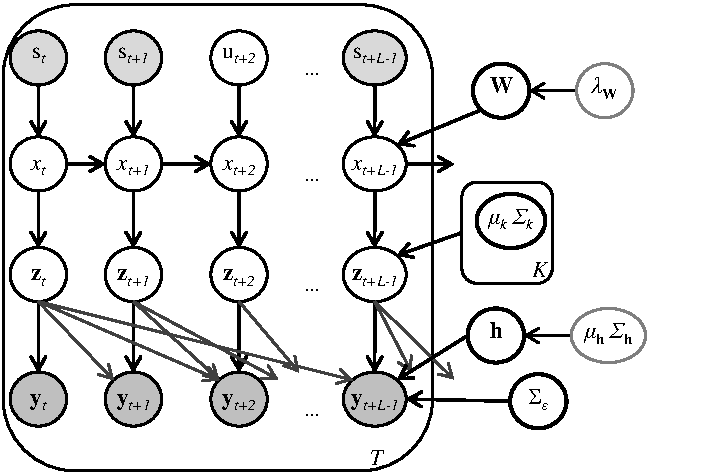
\includegraphics[width=.75\linewidth]{model}
    \caption[The State--Space Model (SSM)]{\textbf{The State--Space Model (SSM).
    } The experimental parameters are represented by $\s_t$,
    while the corresponding brain--state is $\X_t$, and
    the instantaneous activation pattern is $\Z_t$.
    The activation pattern is observed in the fMRI data $\Y_t\ldots
    \Y_{t+L-1}$  after convolution with the HRF $\h$.
    \label{fig:model}
    }
\end{figure}


A certain amount of information about the experimental paradigm can
be provided as input to the SSM estimation routines, in order to
stabilize estimation and provide a reference for estimating the
model hyper-parameters (using prediction error, measured through
cross-validation). In general, if an experiment has multiple types
(channels) of stimuli and subject responses prevalent during its
course, only some of these channels may be included in the model
estimation, as necessary. The effect of the remaining experimental
parameters on the SSM can be tested post-hoc, i.e.~after the model
has been estimated. The reader is referred to
\cite{Janoos2010g,Janoos2011} for more details on this.

\section{Specifying the Experimental Design}
\label{sec:specify}
The experimental design, to be provided as input to the
model-specification, is specified using the \verb"Specify 1-st Level"
feature of SPM (\cf.~\Fig ). Please refer to the SPM
Manual~\cite{TheFILMethodsGroup2011} for more details.

Of interest are the different conditions, their presentation timing
and duration. The rest of the fields may be filled with filler or
dummy values. Save the \verb"Specify 1-st Level" batch job as a
\verb".mat" file. This \verb".mat" is provided as input the SSM
estimation routine. There is no need to run the job - as the
\verb"SPM.mat" containing the design matrix \emph{is not used}.

\begin{figure}
\centering
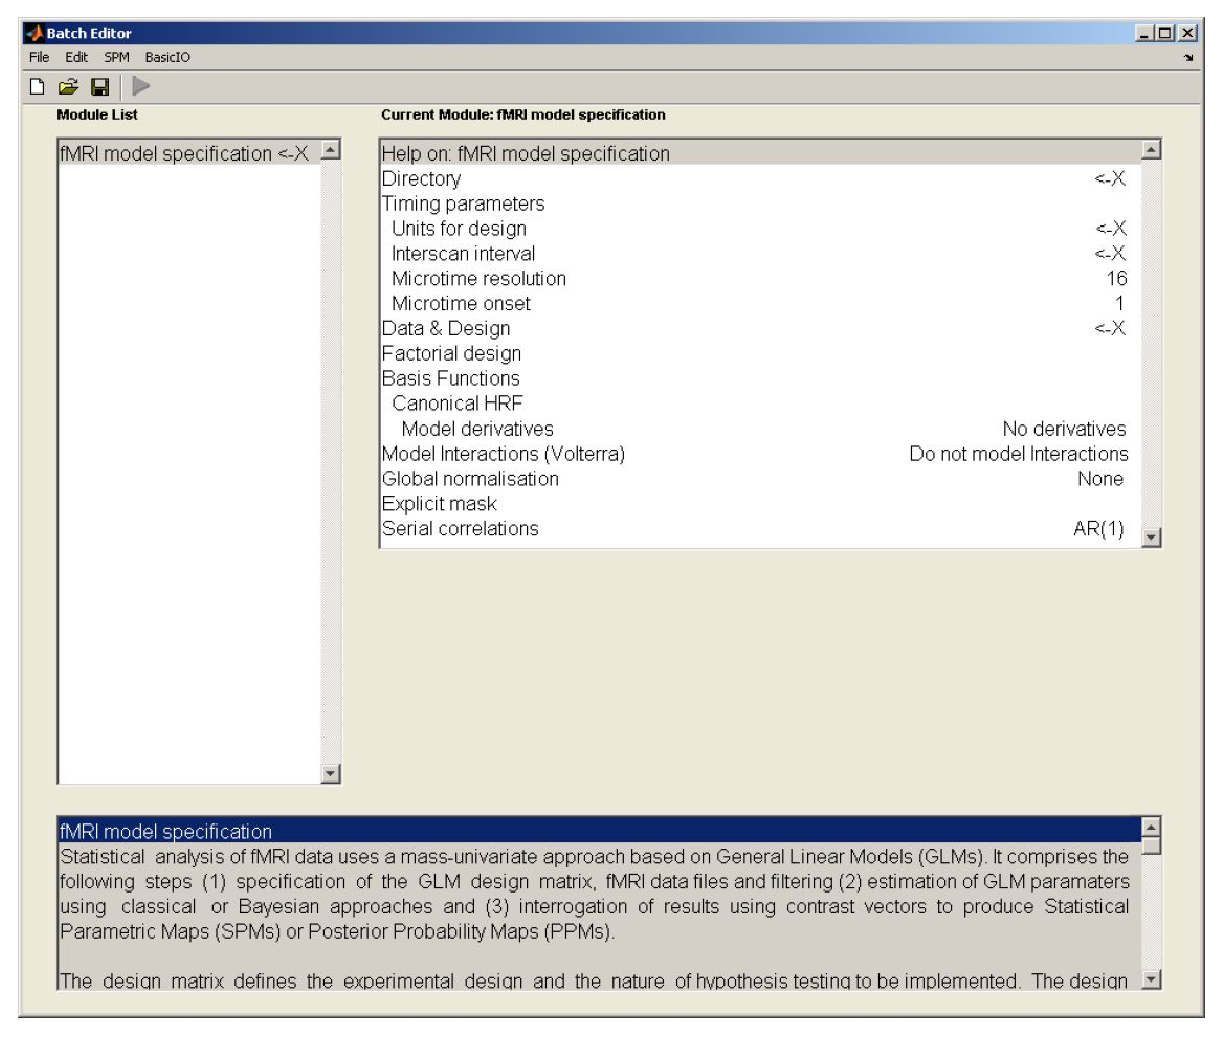
\includegraphics[width=.75\linewidth]{spm-specify}
    \caption[Specifying the Experimental Design.]
    {\textbf{Specifying the Experimental Design.}
    Use the ``Specify 1-st Level'' of SPM to specify the
    experimental conditions and the timing.
    \label{fig:specify}
    }
\end{figure}

%%  \item The length of a block of missing stimuli (in TR units)
%%  for the cross validation method of hyper-parameter selection
%%  \item The number of cross-validation iterations


\section{Estimating the Model}

To estimate the model, and do hyper-parameter selection, the following function
is used:

Function Syntax:
\begin{verbatim}
    [error_missing, log_likelihood, params_opt ]
        = ssmEstimateFull(fs_coords, specify_mat_file,
                          num_cvs, block_length,
                          tol);
\end{verbatim}
Arguments:
\begin{itemize}
  \item \verb"fs_coords" - The feature-space embedding of the fMRI session
  \item \verb"specify_mat_file" - The name of the \verb"Specify 1-st spm Level"
   job batch file (\verb".mat" format) created in \Sec{sec:specify}.
  \item \verb"num_cvs" - (Optional, Default 5) Number of cross validation steps for hyper-parameter selection.
  Typically set between 5--10.
  \item \verb"block_length" - (Optional, Default 5)  The length of a block of missing stimuli (in TR units)
     for the cross validation method of hyper-parameter selection. Typically set
     between 4 -- 8.
  \item \verb"tol" - (Optional) The relative tolerance of the various
  parameter updates specifying the termination criteria for iterative optimization. Typically
  set at 0.001 (indicating termination for a 0.1\% change in parameter value).
\end{itemize}`
Returns:
\begin{itemize}
    \item \verb"error_missing" - An array giving the distribution of the missing stimulus prediction
    error rate (over multiple cross validations) for the optimal model.
    \item \verb"log_likelihood" - An array giving the distribution of the data log
    likelihood (over multiple cross validations) for the optimal model.
    \item \verb"params_opt" - A structure of the SSM parameters averaged multiple CVs for the optimal model.
    It contains the fields:
    \begin{itemize}
      \item \verb"K_opt" - Optimal model size (number of states).
      \item \verb"lambda_opt" - Optimal value of the hyper-parameter controlling the
      estimation of the state-transition    parameters.
      \item \verb"lambda_opt" - Optimal value of the hyper-parameter controlling the
      estimation of the state-transition    parameters.
      \item \verb"w" - The 3-d array giving the state transition parameters $\mathbf{w}$,
      where \verb"w(i,j,:)" = $\mathbf{w}_{i,j}$.
      \item \verb"omega" - The 2-d array giving the state transition parameters $\omega$,
      where \verb"omega(i,:)" = $\omega_{i}$.
      \item \verb"mu" - An 2-d matrix where each column gives the mean value of the activation
      patterns corresponding to each state.
      \item \verb"Sigma" - An 3-d matrix where each 2-d sub-matrix gives the variance for each state.
      \item \verb"h" - An 2-d matrix where each column gives the estimated hemodynamic response filter
      for each element of the feature (data embedding) space.
      \item \verb"Sigma_eps" - A 2-d matrix giving the noise variance in the activation patterns.
    \end{itemize}
\end{itemize}

It is also possible to estimate the model for a given setting of the
hyper-parameters, and a given subset of the stimulus marked as hidden (unobserved) using the function described
next:
Function Syntax:
\begin{verbatim}
    [error_missing, log_likelihood, params ]
        = ssmEstimate(fs_coords, specify_mat_file,
                          t_missing, K, lambda,  tol);
\end{verbatim}
Arguments:
\begin{itemize}
  \item \verb"t_missing" - A vector of binary values the length of the session with $1$ indicating which time-point to treat
  as missing / hidden stimulus.
\end{itemize}`


\chapter{Model Exploration}
\label{chap:explore}
%model-explore.v1

The spatio-temporal SSM encodes information about the abstract state
of the subject, the spatial maps corresponding to the state, the
state transition probabilities, and the hemodynamic response. In
addition, the optimal state-sequence for a particular fMRI session
(not necessarily the same as the one against which the SSM
parameters were estimated) can also be computed.

The \verb"params" object returned by \verb"ssmEstimateFull" (or by
\verb"ssmEstimate" encapsulates all the parameters of the SSM, which
can be explored by MATLAB code fragments. Addition, some helper
functions have also been provided, listed below.


\section{Computing Optimal State-Sequence}

This function estimates the optimal state-sequence by a specific
model for a given fMRI session.

Function Syntax:
\begin{verbatim}
    [st_seq_opt, log_likelihood ]
        = ssmGetStateSeq(params, fs_coords_session);
\end{verbatim}
Arguments:
\begin{itemize}
  \item \verb"params" - A structure of the SSM parameters as
  defined earlier.
  \item \verb"fs_coords" - The feature-space embedding of the fMRI session
\end{itemize}`
Returns:
\begin{itemize}
    \item \verb"st_seq_opt" - An array
    \item \verb"log_likelihood" - The log likelihood of the optimal
    state sequence
\end{itemize}


\section{State Marginal Distribution}
It is possible to compute the marginal probability distribution of
each state conditioned on a specific stimulus $\Pr[\x_t = k | \s_t]$
as follows

Function Syntax:
\begin{verbatim}
    [log_marginal ]
        = ssmStateMarginal(params, cond);
\end{verbatim}
Arguments:
\begin{itemize}
  \item \verb"params" - A structure of the SSM parameters as
  defined earlier.
  \item \verb"cond" - A structure giving the value of each stimulus
  (experimental conditions) for which the
  marginal is desired. Stimuli omitted from this structure are
  marginalized out. For example, let the names of the conditions
  as given in the \verb".mat" file created during
  the \verb"Specify 1-st Level" batch job of SPM,
  be \verb"stimulus_1" ... \verb"stimulus_n". If the distribution of
  state probabilities for \verb"stimulus_1"=5, \verb"stimulus_3"=2 are
  required, regardless of the other stimuli, then \verb"cond" will
  be
\begin{verbatim}
    cond.stimulus_1 = 5;
    cond.stimulus_3 = 2;
\end{verbatim}

\end{itemize}`
Returns:
\begin{itemize}
    \item \verb"log_marginal" - An array giving the log marginal probabilities for
    each state, under the specified experimental conditions.
\end{itemize}

This function can be used to generate plots giving the distribution
of each state during different experimental conditions, as shown in
\Fig{fig:state-trans}
\begin{figure}
     \centering
    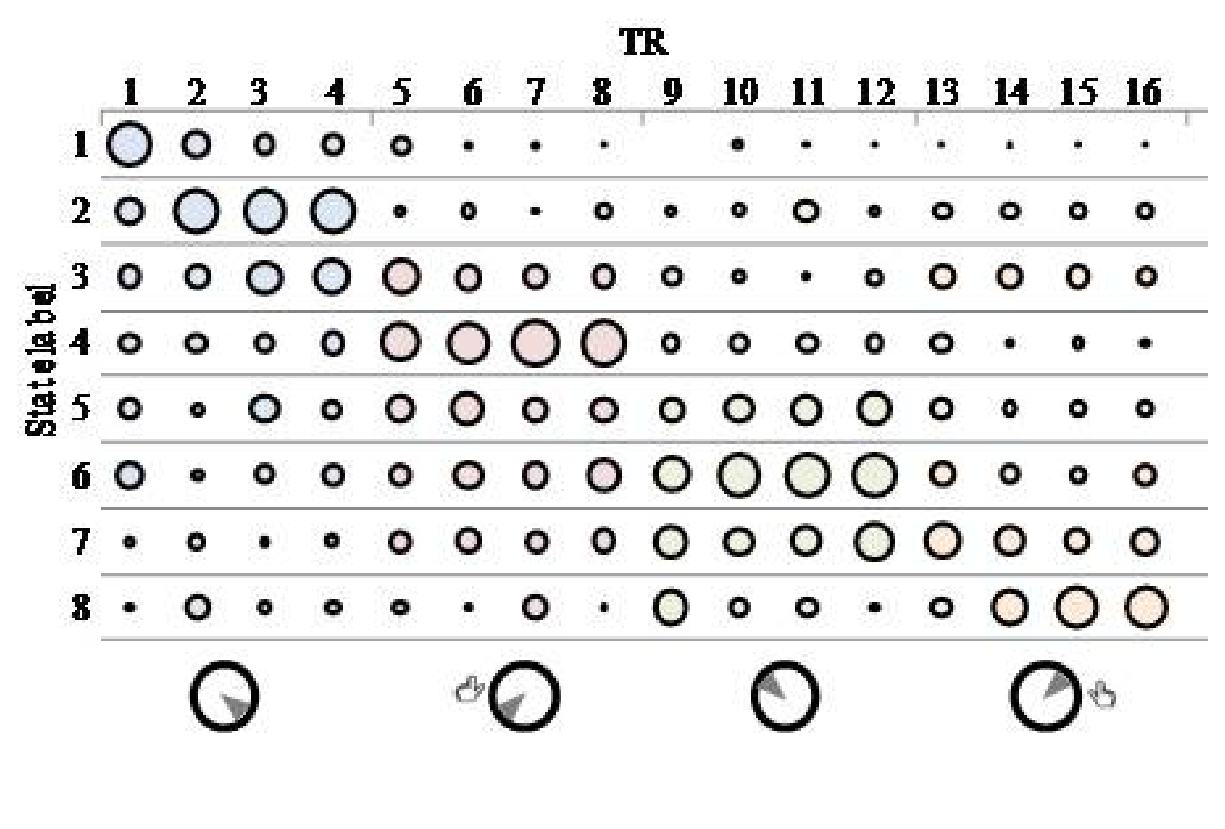
\includegraphics[width=\linewidth]{state-transition}
     \caption[Brain--State Probabilities]
     {\textbf{Brain--state probabilities for one subject.}
     The size of the
     circles corresponds to the marginal probabilities
     of the states during the display of the wedge in lower right,
     lower left, upper left and upper right quadrants for 4TRs each.
     States have been relabeled for expository purposes and
     transition probabilities have been omitted for visual clarity.}
    \label{fig:state-trans}
    \vspace{-.3cm}
\end{figure}


\section{Obtaining the State Transition Distribution}
Similar to the method above, it is possible to compute the entire
state transition probability matrix, conditioned on a specific
stimulus $\Pr[\x_{t} = j| \x_{t-1} = i , \s_t]$ as follows

Function Syntax:
\begin{verbatim}
    [log_transition]= ssmStateTransition(params, cond);
\end{verbatim}
Arguments:
\begin{itemize}
  \item \verb"params" - A structure of the SSM parameters as
  defined earlier.
  \item \verb"cond" - A structure giving the value of each stimulus
  (experimental conditions) for which the
  marginal is desired, as describe above.
\end{itemize}
Returns:
\begin{itemize}
    \item \verb"log_transition" - An 2D array giving the
    log probabilities for a state transition from
    state $i$ (row index) to state $j$ (column index),
    under the specified experimental conditions.
\end{itemize}





\section{The Activation Maps}
The spatially distributed activation pattern for a specific value of
the experimental variables along with its $z$--score map is computed
using the next function.

Function Syntax:
\begin{verbatim}
    [act_map_vi, z_map_vi ]  = ssmActivationMap(params, cond,
                            basis_set_idx, basis_filename);
\end{verbatim}
Arguments: Arguments:
\begin{itemize}
     \item \verb"params" - A structure of the SSM parameters as
      defined earlier.
  \item \verb"cond" - A structure giving the value of each stimulus
  (experimental conditions) for which the
  marginal is desired, as describe above.
    \item \verb"basis_set_idx" -
   The indices of the basis vector of the feature-space that
   retained after dimensionality reduction (\cf \Sec{sec:basc})
  \item \verb"basis_filename" -
    The filename of the 4D zipped NII (\verb".nii.gz")
    containing the basis vectors computed for a particular re-sample of the
    session.
\end{itemize}
Returns:
\begin{itemize}
    \item \verb"act_map_vi" - An \verb"spm_vol" structure giving the
    desired   activation map. Filename format is\\
    \verb"act_map_<cond_name_1>=<value>...<cond_name_n>=<value>.nii"
    \item \verb"z_map_vi" - An \verb"spm_vol" structure giving the
    desired   $z$-score map. Filename format is\\
    \verb"z_map_<cond_name_1>=<value>...<cond_name_n>=<value>.nii"
\end{itemize}
These $z$-score maps can be then examined and visualized either
volumetrically, or on inflated cortical surfaces (using FreeSurfer,
for example) as shown in \Fig{fig:mq-maps}.


\begin{figure}
%\begin{figure}%[h]
\centering
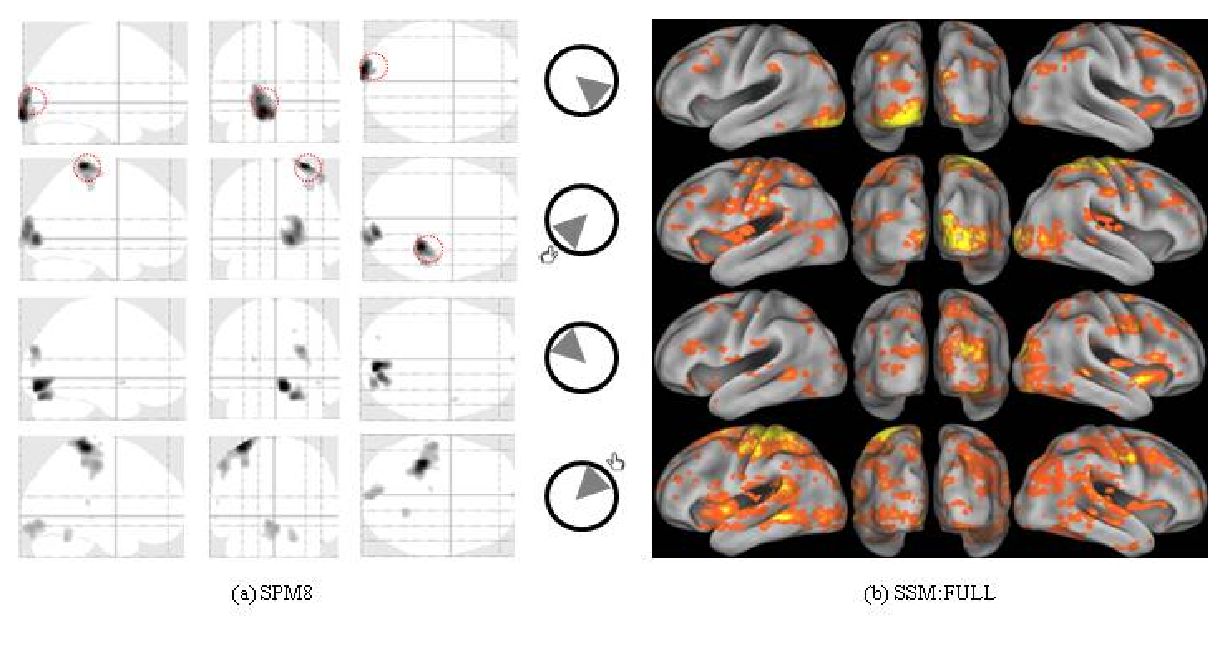
\includegraphics[width=\linewidth]{mq-maps}
\caption[Spatial Activation Maps ]{\textbf{Spatial Activation Maps
for the Visuo-Motor Task from SPM8 and the State--Space Multivariate
Analysis.} Fig.~(a): Maximum intensity projections of significantly
activated voxels ($p < 0.05$, FWE corrected) in a single subject for
the four orientations of the wedge and the hand motor actions,
computed using SPM8. The red circles indicate the ROIs for which the
estimated HR FIR filters are displayed in \Fig{fig:hrf-estimate}.
Fig.~(b): Spatial ($z$--score) maps showing the distribution of
activity for each orientation of the wedge computed from our
state--space model displayed on an inflated surface of the brain.
Displayed are the posterio-lateral and posterio-medial views of the
left and right hemispheres respectively. Values of $z \leq 1$ have
been masked out for visual clarity. }
 \label{fig:mq-maps}
\end{figure}



\section{The HRF Filters}
The SSM estimates an HRF filter at each feature-space coordinate.
These HRF estimates can be recombined and transformed back into the
original (physical) space to give the HRF estimated at a specific
location.

Function Syntax:
\begin{verbatim}
    [hrfs]  = ssmGetHRF(params, spatial_ijk,
                            basis_set_idx, basis_filename);
\end{verbatim}
Arguments: Arguments:
\begin{itemize}
     \item \verb"params" - A structure of the SSM parameters as
      defined earlier.
  \item \verb"spatial_ijk" - A $3\times n$ array giving the voxel
  coordinates (in $i-j-k$) at which the HRF estimates are desired.
    \item \verb"basis_set_idx" -
   The indices of the basis vector of the feature-space that
   retained after dimensionality reduction (\cf \Sec{sec:basc})
  \item \verb"basis_filename" -
    The filename of the 4D zipped NII (\verb".nii.gz")
    containing the basis vectors computed for a particular re-sample of the
    session.
\end{itemize}
Returns:
\begin{itemize}
    \item \verb"hrf" - An $n$ item array of the HRF filter
    coefficients for the desired spatial locations.
\end{itemize}

The HRFs can then be visualized as in \Fig{fig:hrf-estimate}


\begin{figure}[h!]
     \centering
 \mbox{
   \subfigure[Motor Cortex ROI]{
   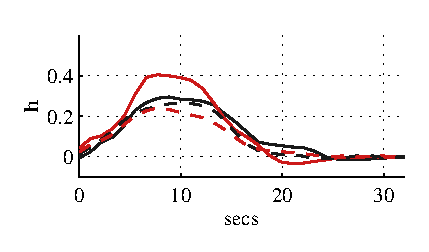
\includegraphics[width=0.5\linewidth]{hrf_motor}
   }
    \subfigure[Visual Cortex ROI]{
    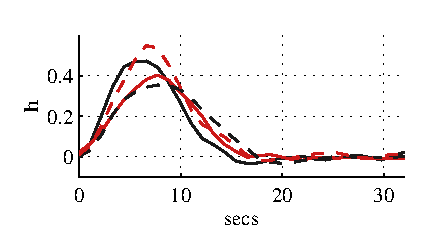
\includegraphics[width=0.5\linewidth]{hrf_visual}
    }
}
    \caption[Estimated Hemodynamic Response]
    {\footnotesize \textbf{Estimated hemodynamic FIR filter $\h$.}
    The estimated FIR filter coefficients for each of the four
    subjects averaged in two ROIs selected in the motor and visual cortices.
    \label{fig:hrf-estimate}
    }
\end{figure}


%\appendix

%------------------------------------------------------------------------------
%\part*{References}
%------------------------------------------------------------------------------
\bibliographystyle{apalike}
\addcontentsline{toc}{part}{References}
\bibliography{library}
%;D:/docs/library

\end{document}
